%% Submissions for peer-review must enable line-numbering 
%% using the lineno option in the \documentclass command.
%%
%% Preprints and camera-ready submissions do not need 
%% line numbers, and should have this option removed.
%%
%% Please note that the line numbering option requires
%% version 1.1 or newer of the wlpeerj.cls file, and
%% the corresponding author info requires v1.2

\documentclass[fleqn,10pt,lineno]{wlpeerj} % for journal submissions
%\documentclass[fleqn,10pt]{wlpeerj} % for preprint submissions

\graphicspath{ {./figures/} }% Path to figure files
\usepackage{rotating} % for rotating the graphics 90 degrees


\title{Implementation of Adaptive Integration Method for Free Energy Calculations in Molecular Systems}

\author[1]{CA Mirabzadeh}
\author[2]{FM Ytreberg}
\affil[1,2]{Department of Physics, University of Idaho, Moscow ID}

\corrauthor[2]{FM Ytreberg}{ytreberg@uidaho.edu}

% \keywords{Keyword1, Keyword2, Keyword3}

\begin{abstract}
Estimating free energy differences by computer simulation is useful for a wide variety of applications such as virtual screening for drug design and for understanding how amino acid mutations modify protein interactions. However, calculating free energy differences remains challenging and often requires extensive trial and error and very long simulation times in order to achieve converged results. Here, we present an implementation of the adaptive integration method (AIM). We tested our AIM implementation on two molecular systems and compared results from AIM to those from a suite of standard methods. The model systems tested here include calculating the solvation free energy of methane, and the free energy of mutating the peptide GAG to GVG. We show that AIM is more efficient than standard methods for these test cases, that is, AIM results converge to a higher level of accuracy and precision for a given simulation time.
\end{abstract}

\begin{document}

\flushbottom
\maketitle
\thispagestyle{empty}

\section*{Introduction} \label{introduction}

Measuring free energy differences using computer simulations can be computationally expensive, yet is useful for many different applications (see e.g., \cite{SteinBrecher2010,Chodera2011a,Mobley2013,Zhan2013,Miller2014,Petukh2015,Zhan2015,Wichman2016,Cournia2017}). Specific examples include determining protein conformational preferences or virtual screening for drug design \citep{Zhan2015, SteinBrecher2010, Chodera2011a}. Of specific relevance to the current study is that free energy calculations allow prediction of how amino acid mutations may modify protein-protein binding \citep{Zhan2013, Miller2014, Petukh2015, Wichman2016}. We are particularly interested in developing and implementing efficient methods for calculating free energy differences and using them to understand how amino acid mutations modify protein-protein and protein-substrate interactions. 

For this report, we have implemented the adaptive integration method (AIM), introduced by \cite{Fasnacht2004}, for use in the GROMACS \citep{Berendsen1995} molecular dynamics simulation package. Though there are many free energy methods for molecular systems (see e.g., \cite{Lyubartsev1996,Goncalves2004, Kofke2005, Shirts2007, Chodera2011, Klimovich2015}), in previous studies AIM has shown promise to provide high quality, precise and efficient estimates of binding free energies\citep{Ytreberg2006, Kaus2014}. AIM is an adaptive sampling method that continuously improves the estimate for free energy during the simulation. AIM uses Metropolis Monte Carlo to sample $\lambda$ space in order to obtain numerical estimates of the free energy differences. The algorithm automatically increases sampling in regions where this is needed along the reaction pathway.

For comparison with other free energy methods we used the Python tool, alchemical-analysis.py \citep{Klimovich2015}, part of the Pymbar package \citep{Shirts2008}. The alchemical-analysis tool takes the output from molecular dynamics simulations and estimates the free energy using some standard methods, including the Bennett acceptance ratio, multistate Bennett acceptance ratio, thermodynamic integration and exponential averaging. 
The most substantial difference between these methods and AIM is that they all expect equilibrium sampling of configurations for each $\lambda$. This is achieved via fixed-$\lambda$ standard molecular dynamics simulations, instead of the Monte Carlo $\lambda$ moves used in AIM.

For the current study we chose two molecular systems that have well-documented results and are important starting points for biomolecular free energy studies. First, we calculated the solvation free energy of methane. Simulations were performed and the free energies were calculated using the standard methods provided by alchemical-analysis. Simulations were also performed using AIM and results compared to standard simulations. Using the lessons learned from the methane system, we then calculated the free energy of mutating GAG to GVG in water. For both systems, we found that AIM produces free energy estimates that are within statistical uncertainty of standard methods but with greater efficiency (i.e., more accurate for a given simulation time).

\section*{Methods} \label{methods}

For this study we performed alchemical free energy simulations where the system is changed from a reference state to an end state by constructing a reaction pathway that either adds or removes a small molecule of interest. Such alchemical simulations are non-physical, i.e., the simulation does not represent what could occur naturally. Since the free energy is a state variable, it is independent of the path taken, and we are free to provide any path we wish. To perform these simulations the reaction pathway is divided into many separate, non-physical, $\lambda$ states between a reference state and an end state. The $\lambda$ states represent the progression along a reaction pathway as the reference state transforms into the end state. 

Like most methods used to calculate free energies we start from the free energy identity,
\begin{equation}\label{eq:free_id}
    F = U - TS,
\end{equation}
where $U$ is the potential energy, $T$ is the temperature and $S$ is the entropy of the system.
For free energy differences we generalize the formulation of the change in free energy by separating calculations into two, non-overlapping, thermodynamic end states, $A$ and $B$, at constant system temperature $T$,
\begin{equation}
    \Delta F \equiv \Delta F_{A \rightarrow B} = F_{B} - F_{A}= \Delta U - T \Delta S.
\end{equation}
$\Delta F$ is the change in free energy, $\Delta U$ is the change in potential energy and $\Delta S$ is the change in entropy of the system.
According to statistical mechanics, the free energy difference between the two end states, A and B, of the system is the log of the ratio of probabilities related to the energy states, $U_{A}(\vec{x})$ and $U_{B}(\vec{x})$,
\begin{equation}\label{eq:free}
    \Delta F = -k_{B}T \ln{\frac{Z[U_{B}(\vec{x})]}{Z[U_{A}(\vec{x})]}}.
\end{equation}
Here, $k_{B}$ is the Boltzmann constant and $Z[U(\vec{x})]$ is the partition function for the energy states, $U_{A}(\vec{x})$ and $U_{B}(\vec{x})$, where $\vec{x}$ is the vector of configuration coordinates,
\begin{equation}\label{eq:part}
    Z[U(\vec{x})] = \int \exp{(-\beta U(\vec{x})}) \; dx,
\end{equation}
and $\beta = \frac{1}{k_{B}T}$.

Computationally, we calculate free energy differences between end states by sampling molecular dynamics simulations along a reaction pathway of intermediate states, defined by $\lambda$, such that,
\begin{equation}
    0 \leq \lambda \leq 1.
\end{equation}
This pathway connects the two end states of the system. In the case of poor overlap, where the end states may be separated by a high energy barrier, $|U_{B} - U_{A}| \gg k_{B}T$, this pathway mitigates the otherwise very slow convergence of free energy estimates \citep{Shirts2007}. Care should be taken when choosing intermediate states such that there is adequate overlap in the conformation space between the end states \citep{Shirts2007, Klimovich2015}. For our simulations the number of $\lambda$ values and time per $\lambda$ were chosen through extensive trial and error (more on this below). With proper intermediate states, we are now able to calculate the free energy difference between the two end states. 

The method of exponential averaging \citep{Zwanzig1954} starts from Eq.\ (\ref{eq:free}) above and then adding and subtracting $\exp{(-\beta U(\vec{x}))}$ from the integral in the partition function of the numerator we end up with the final relationship,
\begin{equation}\label{eq:exp}
    \Delta F = -k_{B}T \ln \langle \exp{(-\beta U(\vec{x}))} \rangle.
\end{equation}
where $\langle\cdot\rangle$ represents an average of the equilibrium configuration for $\lambda$
Unlike some other methods, exponential averaging has an exact solution since it is only used to evaluate the difference between two states. However, it is the least efficient method and should not be used if difference in potential energies are much larger than $k_{B}T$ \cite{Shirts2005}.
In addition, exponential averaging can be noisy, biased and dependent on the tails of the distribution of $\lambda$ states \citep{Bruckner2011,Shirts2005}.

The Bennett \citep{Bennett1976} and multistate \citep{Shirts2008} Bennett acceptance ratio (BAR and MBAR) methods are far more efficient than exponential averaging and are commonly used to avoid the shortcomings of other methods \citep{Shirts2005, Ytreberg2006}. BAR and MBAR typically achieve the same statistical precision as TI with fewer $\lambda$ states unless the integrand for TI is very smooth \citep{Monticelli2013, Ytreberg2006}. The complete derivation can be found in Bennett's paper \citep{Bennett1976} but the premise is; for sufficiently large samples $n_{i}$ of $U_{i}$ and $n_{j}$ of $U_{j}$,
\begin{equation}\label{eq:bar}
    \Delta F(i \rightarrow j) = k_{B}T \ln{\frac{\langle f(\Delta U_{ij} + C) \rangle_{j}}{\langle f(\Delta U_{ji} - C) \rangle_{i}}} + C.
\end{equation}
C is a shift constant,
\begin{equation}\label{eq:barc}
    C = k_{B}T\ln{\frac{n_{j}}{n_{i}}},
\end{equation} 
and $f(x)$ is the Fermi function,
\begin{equation}\label{eq:fermi}
    f(x) = \frac{1}{1 + \exp(\beta x)}. 
\end{equation}
Equation\ (\ref{eq:bar}) is the ratio of canonical averages of two different potentials $U_{i}$ and $U_{j}$ acting on the same configuration space meaning it requires information from two neighboring states. However, this limitation is not too much of a concern with a trivial coordinate transformation or when using dummy coordinates in alchemical simulations. MBAR, an extension of BAR, differs in that it takes data from more than two states hence the name "multistate".

For thermodynamic integration (TI) we estimate the free energy by first looking at the derivative of Eq.\ (\ref{eq:free_id}) with respect to $\lambda$,
\begin{equation}\label{eq:diffeq}
    \frac{\partial F}{\partial \lambda} = \left< \frac{\partial U}{\partial \lambda} \right>_{NVT}.
\end{equation}
This differential equation, Eq.\ (\ref{eq:diffeq}), can then be integrated to give,
\begin{equation}\label{eq:ti}
    \Delta F = \int_{\lambda = 0}^{1} \left< \frac{\partial U_{\lambda}(\vec{x})}{\partial \lambda} \right>_{\lambda} d\lambda
\end{equation}
where the $\langle \cdot \rangle_{\lambda}$ notation represents the ensemble average at a given intermediate state, $\lambda$. The free energy is estimated by numerically integrating Eq.\ (\ref{eq:ti}) after running equilibrium simulations at each intermediate $\lambda$ state. Since numerical integration is required, TI can be biased by the chosen method of integration. Some of that bias can be removed by using cubic-spline interpolation or more complex integration estimators\citep{Shirts2005, Shyu2009}.

AIM is similar to TI in that numerical integration of Eq.\ (\ref{eq:ti}) is performed; the key difference is how $\lambda$ space is sampled. AIM uses Metropolis Monte Carlo to move in $\lambda$ space. In AIM, a random move from $\lambda_{old}$ to $\lambda_{new}$ is accepted with probability
\begin{equation}\label{eq:aimaccept}
\min\{1,\exp(- \beta( U_{new} - U_{old})+\beta(F_{new} - F_{old})\}
\end{equation}
where $U_{new} - U_{old}$ is the difference in the potential energy for the old and new $\lambda$ values. $F_{new} - F_{old}$ is the estimated free energy difference based on the current running averages of $\frac{dU}{d\lambda}$.

\subsection*{Implementation} \label{implementation}

AIM was implemented into GROMACS as an expanded ensemble calculation; the Hamiltonian must be calculated along with its derivative, and an expanded ensemble step must be performed for every dynamics step. In GROMACS, \texttt{nstexpanded} is the number of integration steps between attempted $\lambda$ moves changing the system Hamiltonian in expanded ensemble simulations. This value must be a multiple of \texttt{nstcalcenergy}, the number of steps before calculating the system energy, but can be greater or less than \texttt{nstdhdl}, the number of steps before calculating $\frac{dU}{d\lambda}$ (referred to as dHd$\lambda$ in GROMACS documentation). For a detailed explanation of all technical terms see: \cite{gmxmanual}. The GROMACS package was further altered to print out the $\frac{dU}{d\lambda}$ averages computed by AIM to the log file when AIM is used as the \texttt{lmc-mover}.

AIM requires the $\frac{dU}{d\lambda}$ value from every dynamics step to be stored regardless of whether a move in $\lambda$ space is attempted. Since $\frac{dU}{d\lambda}$ is only calculated at each step where free energies are calculated, every \texttt{nstdhdl} step, we set \texttt{nstexpanded} = \texttt{nstdhdl} = \texttt{nstcalcenergy} = 1 for AIM simulations. This further implies that \texttt{lmc-stats} functions were not used during AIM simulations because those functions modify the Hamiltonian which is counter intuitive for AIM as the algorithm requires the derivative of the unmodified Hamiltonian. Making a comparison between a modified Hamiltonian and its unmodified derivative would require re-weighting which introduces statistical noise and is entirely impractical.

For the implementation of AIM with GROMACS we follow the outline given in our previous study, \cite{Ytreberg2006}. 
\begin{enumerate}
\item Start the simulation from an equilibrated configuration at $\lambda$=0 and perform one molecular dynamics step. 
\item Randomly choose a trial move in $\lambda$ space. For example, if our $\lambda$ spacing is 0.05, a move from $\lambda$=0.35 to 0.4 or 0.3 may be attempted but not to 0.45. 
\item Calculate the difference in potential energy between $\lambda$ trial and $\lambda$ current.
\item Estimate the free energy difference between the running average of $\lambda$ trial and the running average $\lambda$ current using the trapezoidal rule. 
\item Accept $\lambda$ trial with probability given in Eq.\ \ref{eq:aimaccept}.
\item If the move is accepted then $\lambda$ is updated to the trial value, otherwise the simulations stays at current $\lambda$.
\item The running average of the free energy at $\lambda$ is updated.
\end{enumerate}

\subsection*{Simulation Details} \label{details}

All simulations described in this paper were performed using the molecular dynamics package GROMACS 5.1.4. The simulations were carried out at 300 K and solvated in a dodecahedron box with TIP3P waters. The molecule was parameterized using the OPLS (Optimized Potential for Liquid Simulations) force field \citep{Jorgensen1996}. The OPLS force field was chosen for this study because it is known to perform well on small molecules \citep{Shirts2003}. In future studies, we anticipate using AIM on protein systems where other force fields are more appropriate such as AMBER \citep{Salomon-Ferrer2013} and CHARMM \citep{Mackerell2001}. Since all molecular dynamics force fields have similar form and number of parameters, it is expected that the performance of AIM would not depend on the force field chosen. 

For the GAG to GVG mutations, NaCl ions were added to keep the simulation box neutral and reach a physiologically relevant 150 mM salt concentration. Energy minimization was performed using steepest descent for 1000 steps. The system was then equilibrated using simulated annealing for 1000 ps to heat the system from 100K to 300K. For production simulations, electrostatic interactions were handled by Reaction field with a cut-off of 0.9 nm, Potential-shift-Verlet modifier and Verlet cutoff scheme. Van der Waals interactions were handled by twin range cutoffs with neighbor list cutoff of 1.15 nm and van der Waals cutoff of 0.9 nm. The hydrogen bonds were constrained with the Shake algorithm, allowing for a longer time step of 2 fs. Long range dispersion corrections for energy and pressure were applied. 

For the standard methods we ran fixed $\lambda$ alchemical simulations. For AIM we ran expanded ensemble alchemical simulations. During alchemical simulations we first take a molecular dynamics step, where we calculate the inter-atomic forces and other states of the system. We then take a step in $\lambda$ space where we can apply transformations against the system state. Fixed $\lambda$ simulations spend a fixed amount of time at each intermediate $\lambda$ state. For expanded ensemble methods the amount of time at each intermediate $\lambda$ state is decided by the algorithm.

In order to determine the best distribution of intermediate $\lambda$ states we followed a simple strategy:
(i) Conduct short simulations with a small set of intermediates.
(ii) Generate a plot comparing slope values between AIM and fixed $\lambda$
(iii) Determine the locations of curvature in the estimate of the free energy.
(iv) Increase the density of intermediate states in locations of high curvature.
(v) Repeat until all areas of high curvature have been well explored.

\subsection*{Methane and GAG to GVG Solvation Free Energy} \label{freeenergy}

The first system used here, methane in water, is detailed in systematic studies of force fields and the free energies of hydration of amino acid side chain analogs \cite{Sun1992,Lyubartsev1996,Chodera2011,Paliwal2011}.

For the GAG to GVG mutation the PMX \citep{Gapsys2015} software package was used to construct the tri-peptide mutation. Using PMX, we generated the hybrid protein structure and topology for simulations of the chosen mutation, alanine to valine.

For both of these systems, we calculated the free energy for decoupling the Lennard-Jones interactions between the atomic sites of the molecule of interest in water. For fixed $\lambda$ simulations, separate equilibrium simulations of equal length were run in order to represent each of the intermediate $\lambda$ states. The same values for $\lambda$ were used in both fixed $\lambda$ and AIM expanded ensemble simulations. For fixed $\lambda$ simulations the free energy was estimated using an external tool, alchemical-analysis.py. AIM estimates were calculated using both the trapezoidal rule and cubic-spline. All methods and code may be made available upon request.

\section*{Results} \label{results} 

\subsection*{Methane} \label{res:methane}

After conducting short simulations, generating plots to determine locations of high curvature and increasing $\lambda$ density in those regions, we averaged eight trial simulations of 100 ps per $\lambda$ for separate $\lambda$ distributions, Fig.\ \ref{increasinglambdas}. We found, by progressively increasing the $\lambda$ density between $\lambda$ = 0.5 and $\lambda$ = 1.0, that a distribution of 31 $\lambda$ values gave us a dense enough distribution to properly compare AIM to fixed $\lambda$ methods for the methane simulations.

Fig.\ \ref{methane31} is a violin plot used to visualize the distribution and probability densities over the eight trials for each method as a function of simulation time per value of $\lambda$. A violin plot combines a box plot and a density plot to show the shape of the distribution around the mean. The thick black bar in the center represents the interquartile range, the white dot is the median and the thin black line going vertically through the middle represents the upper and lower adjacent values. Reading a violin plot is similar to reading a density plot. The thicker parts represent high frequency values and the thinner parts represent low frequency values. The advantage of a violin plot over a box plot is that we are able to view the number of clusters in the underlying distribution of the data.

In Fig.\ \ref{methane31}, for 31 $\lambda$ values at 100 ps per $\lambda$, the slower convergence of MBAR leads to two separate distributions of converging points. At 500 ps the other methods are beginning to show signs of convergence, however, we see that AIM is forming a second distribution and the width of the distribution of the other methods has not condensed or flattened along the horizontal axis, suggesting convergence has not yet occurred for any of the methods. Despite this, the average of the methods are in agreement within uncertainty, i.e. variance in the mean of the estimated free energy. At 1 ns per $\lambda$ all methods are similarly converged, indicating the longer simulation times has reduced the variance from the mean. 

\subsection*{GAG to GVG Mutation} \label{res:gxg}

For the GAG to GVG mutation we first tested a distribution of 41 $\lambda$ values averaged over 8 trial simulations of 1 ps and 100 ps per $\lambda$; see Fig.\ \ref{a2vlineplot}. By reviewing the smoothness of the function we concluded that 41 $\lambda$ values was sufficient and continued the simulations for 1 ns per $\lambda$. Fig.\ \ref{a2vviolinplot} shows distribution of the convergence over time for each method. We see that AIM has mostly converged at 100 ps per $\lambda$ and all methods have similarly converged for 1 ns per $\lambda$.

\section*{Discussion} \label{discussion}

In the limit of infinite sampling, all rigorous methods (i.e., statistical mechanics-based methods), performed properly with the same force-field and parameters, will yield the same result within uncertainty. For fixed $\lambda$ simulations the sampling time is typically chosen to be the same for each $\lambda$ state. Thus, we are led to increase sampling time whenever convergence has not been achieved. However, if bias is introduced by using an insufficient number of $\lambda$ values in regions of high curvature, increased sampling leads to radical convergence problems \citep{Shyu2009, SteinBrecher2010}. If the curvature of the underlying free energy function is large, averaging over a state space that is not dense enough to fully describe the state function propagates this bias requiring significantly increased sampling time to achieve convergence. For TI, the bias could persist even for infinite sampling. Increasing sampling time may not be realistic, or beneficial when dealing with limited computational resources. \cite{Paliwal2011} make a detailed argument to why convergence may not be possible for all systems due to hard limitations in computational resources. 

In particular, both TI and AIM are calculating the same slope averages and should agree very well for simple systems and reasonably long simulation times. However, due to the fact that AIM spends more time in some regions, we should not expect the approximation of AIM to exactly match TI with similar sampling time until the number of $\lambda$ values has been sufficiently increased in high curvature regions. Once we have properly chosen the $\lambda$ values then reasonably long simulations should lead to highly similar results between these two methods.

Since AIM is implemented as a Metropolis Monte Carlo \citep{Metropolis1953} expanded ensemble \citep{Lyubartsev1996} method, where the approximation of a given intermediate state is adaptively expanded whenever a better approximation of the state is needed, AIM allows for better sampling as compared to fixed $\lambda$ simulations. AIM is able to smooth the underlying free energy function by spending more time at critical points in the curvature of the Hamiltonian state space. This means that AIM requires fewer $\lambda$ states to fully explore the free energy of a system because we minimize the overall variance of the free energy estimate by adjusting the distribution of data points in each intermediate $\lambda$ state based on the acceptance criteria. This reduces the propagation of error in poorly chosen distributions. 
The observant reader may note that AIM violates detailed balance since the acceptance criterion contains the free energy estimates that are updated continuously. AIM does however obey detailed balance asymptotically. As simulation time increases, the average free energy differences between $\lambda$ values reach an equilibrium and detailed balance is satisfied. 

\section*{Conclusion} \label{conclusion} 

In this report we have implemented the adaptive integration method (AIM) for calculating free energy differences in GROMACS and applied it to two molecular systems. We have shown agreement within statistical uncertainty between AIM and a suite of standard fixed $\lambda$ methods for methane solvation and an GAG to GVG mutation. We have also shown that AIM is more efficient than the other tested methods. That is, for a given amount of simulation time, AIM has a higher level of accuracy and precision compared to other methods.

Further, we found that running longer simulations with too few intermediate $\lambda$ states generated results that were inconsistent between methods. The density and sampling convergence of the $\lambda$ states directly influences the agreement between all the tested methods. Since some states will contribute disproportionately to the variance of the estimate, we found that testing short simulations of different $\lambda$ densities before attempting longer simulations is a more economical use of time and resources.

\section*{Acknowledgments}
Support for this research was provided by the National Science Foundation (DEB 1521049 and OIA 1736253) and the Center for Modeling Complex Interactions sponsored by the National Institutes of Health (P20 GM104420). Computer resources were provided in part by the Institute for Bioinformatics and Evolutionary Studies Computational Resources Core sponsored by the National Institutes of Health (P30 GM103324).

\bibliography{aimrefs}

\pagebreak

\begin{sidewaysfigure}[htbp]
    \centering
    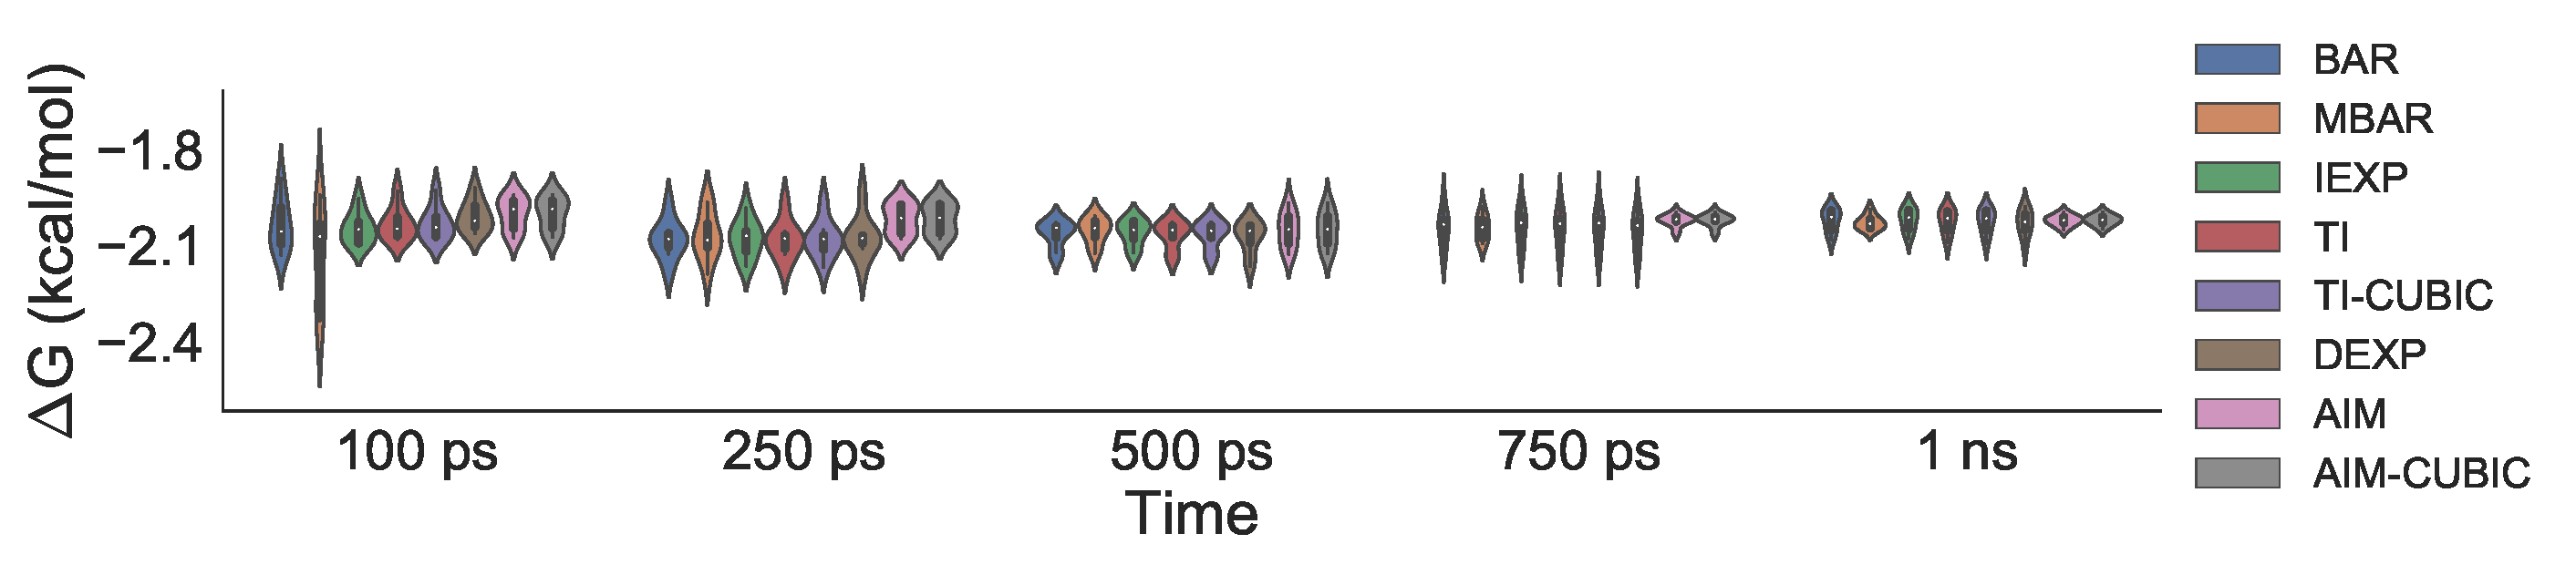
\includegraphics[width=1\textwidth]{Figure_1_Methane_31L_violinplotovertime.eps}
    \caption{\textbf{Violin plot showing methane solvation results for 31 $\lambda$ values averaged over eight trials.} A violin plot combines a box plot and a density plot to visualize the distribution and probability density. The graphic shows all methods have similarly converged at 1 ns per $\lambda$ for the same number of intermediate states and sample size with AIM and AIM-CUBIC showing early convergence at 750 ps per $\lambda$.}
    \label{methane31}
\end{sidewaysfigure}

\pagebreak

\begin{figure}[htbp]
    \centering
    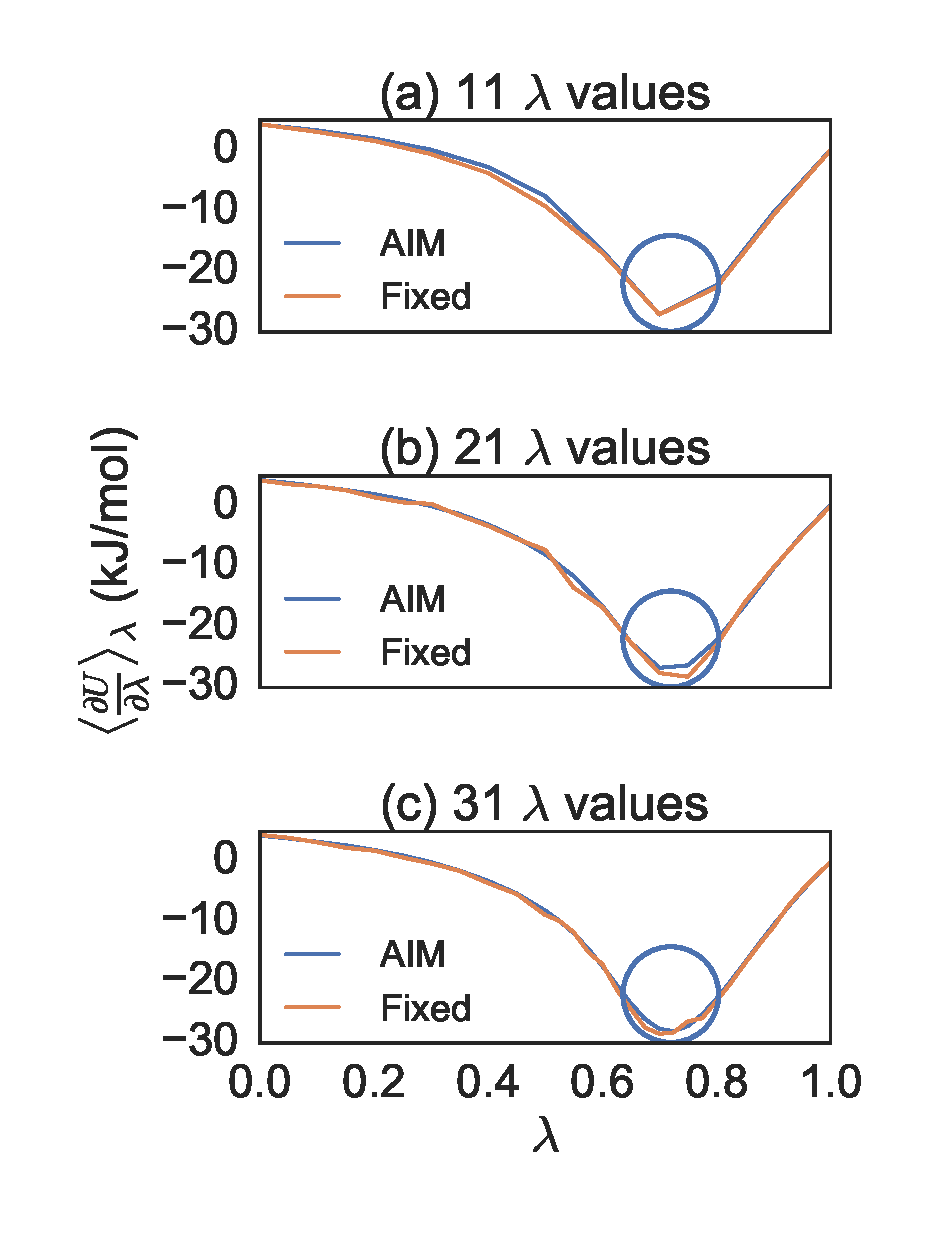
\includegraphics[width=1 \textwidth]{Figure_2_All_lambdas_at_100ps_per_lambda.eps}
    \caption{\textbf{Methane solvation free energy results.} Eight trial simulations of 100 ps per $\lambda$ for 11, 21 and 31 $\lambda$ values. This shows how the number of $\lambda$ values were chosen to effectively compare AIM to fixed $\lambda$ simulations. The circles indicate the region where the $\lambda$ density needed to be increased.}
    \label{increasinglambdas}
\end{figure}

\pagebreak

\begin{figure}[htbp]
    \centering
    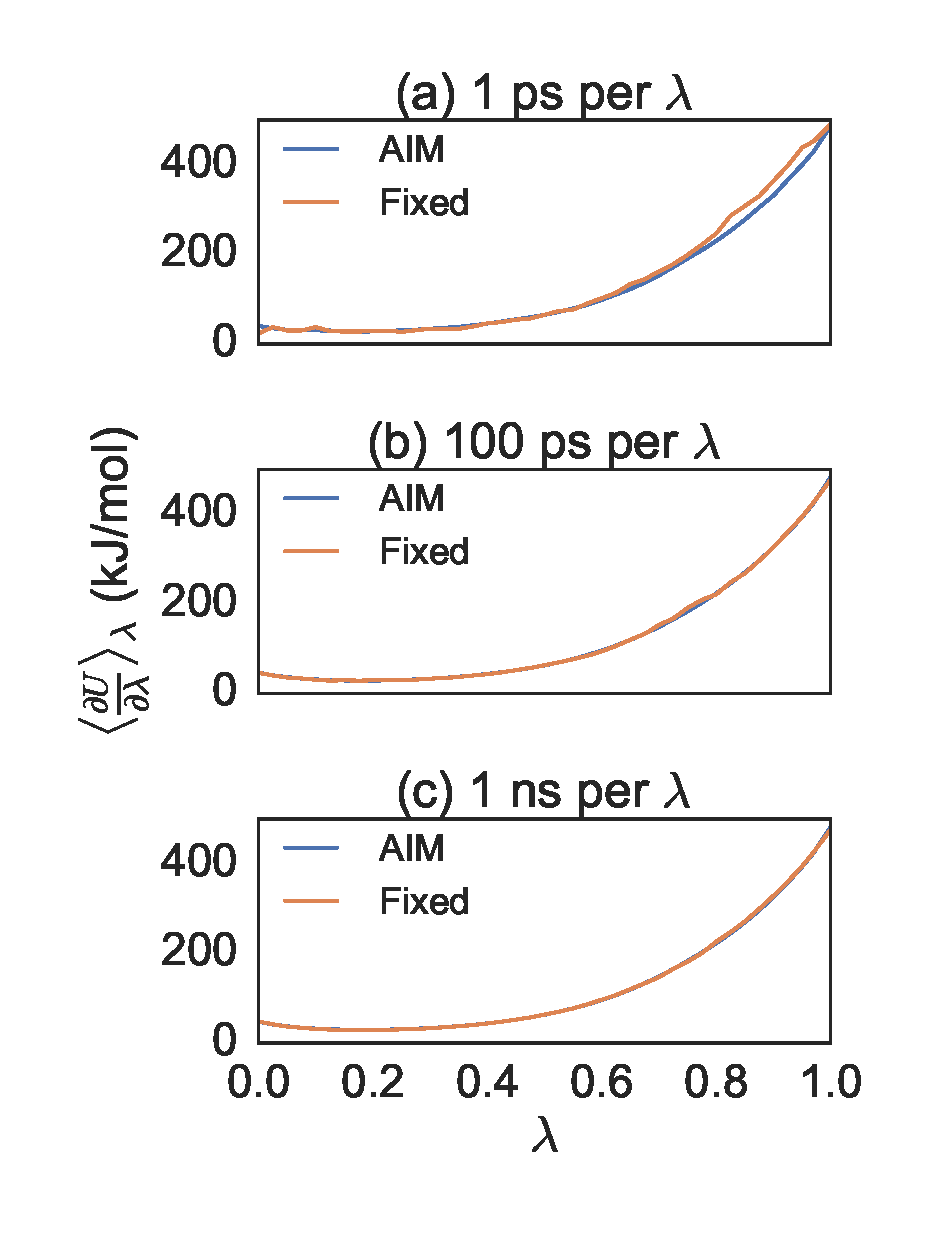
\includegraphics[width=1 \textwidth]{Figure_3_tripep_lambdas.eps}
    \caption{\textbf{Alanine to valine mutation free energy}. Eight trial simulations of 41 $\lambda$ values at 1 ps, 100 ps and 1 ns per $\lambda$. Note the smoothness of AIM versus fixed $\lambda$ simulations. AIM requires less samples than fixed $\lambda$ simulations to smooth the free energy function.}
    \label{a2vlineplot}
\end{figure}

\pagebreak

\begin{sidewaysfigure*}[htbp]
    \centering
    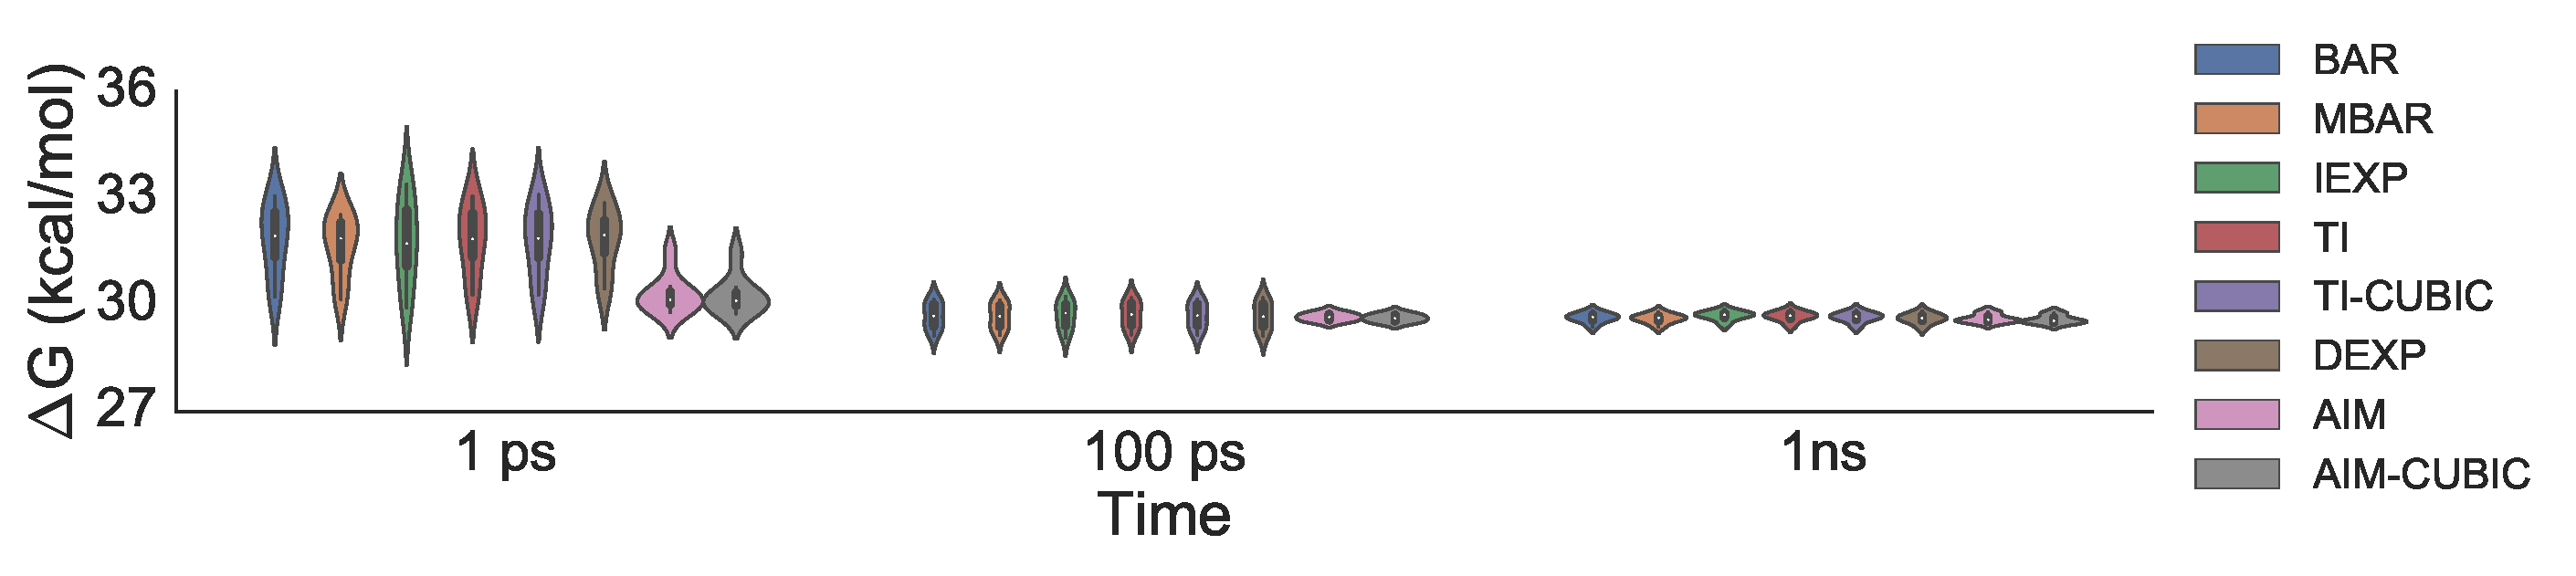
\includegraphics[width=1\textwidth]{Figure_4_A2V_41L_violinplotovertime.eps}
    \caption{\textbf{Violin plot showing alanine to valine mutation results for 41 $\lambda$ values averaged over eight trials}. The graphic shows all methods have similarly converged at 1 ns per $\lambda$. Note that AIM and AIM-CUBIC converge more rapidly than other methods and are mostly converged at 100 ps per $\lambda$}
    \label{a2vviolinplot}
\end{sidewaysfigure*}

\end{document}